\documentclass[11pt,a4paper]{article}
% Sprint 1 Report, COS40005 Group HN_9. Generated from the team's Google Doc; edit here from now on.
\usepackage[T1]{fontenc}
\usepackage[utf8]{inputenc}
\usepackage{lmodern}
\usepackage[a4paper,margin=2.3cm]{geometry}
\usepackage{microtype}
\usepackage{graphicx}
\usepackage{float}
\usepackage{array}
\usepackage{longtable}
\usepackage{booktabs}
\usepackage[table]{xcolor}
\usepackage{caption}
\usepackage{enumitem}
\usepackage{fancyhdr}
\usepackage{titlesec}
\usepackage[hidelinks]{hyperref}
\usepackage{url}

\captionsetup{font=small,labelfont=bf,skip=6pt}
\captionsetup[longtable]{position=top}
\setlength{\parindent}{0pt}
\setlength{\parskip}{0.6em}
\setlist{itemsep=2pt,topsep=4pt}
\renewcommand{\arraystretch}{1.25}
\setcounter{tocdepth}{2}
\titleformat{\section}{\Large\bfseries}{\thesection}{0.8em}{}
\titleformat{\subsection}{\large\bfseries}{\thesubsection}{0.8em}{}
\titleformat{\subsubsection}{\normalsize\bfseries}{\thesubsubsection}{0.8em}{}

\pagestyle{fancy}
\fancyhf{}
\fancyhead[L]{\small COS40005 \textbar{} Group HN\_9}
\fancyhead[R]{\small Sprint 1 Report}
\fancyfoot[C]{\small \thepage}
\renewcommand{\headrulewidth}{0.4pt}

\begin{document}
\begin{titlepage}
\centering
\vspace*{3cm}
{\Huge\bfseries Sprint 1 Report\par}
\vspace{0.6cm}
{\Large Sprint 1 (Week 9)\par}
\vspace{2cm}
\begin{tabular}{>{\bfseries}r l}
Unit code: & COS40005 \\
Unit name: & Computing Technology Project A \\
Group: & HN\_9 \\
Supervisor: & Dr. Le Minh Duc \\
Submission date: & 14/11/2026 \\
\end{tabular}
\par\vspace{1.5cm}
{\bfseries Team members\par}
\vspace{0.3cm}
Nguyen Duc Manh\par
Le Anh Tuan\par
Do Trinh Thuan Minh\par
Nguyen Quoc Trung\par
Nguyen Xuan Doanh\par
\vfill
{\small GitHub repository: \url{https://github.com/Bill2926/COS40005_HN9_Verifiable_Co-Learner_Agent}\par}
\end{titlepage}

\tableofcontents
\clearpage
\section*{Acknowledgement and Report Overview}
\addcontentsline{toc}{section}{Acknowledgement and Report Overview}
\subsection*{Acknowledgement of Country}
\addcontentsline{toc}{subsection}{Acknowledgement of Country}
We acknowledge the Wurundjeri People of the Kulin Nation, the Traditional Owners of the land on which Swinburne's Australian campuses in Melbourne's east and outer east are located. We pay respect to Elders past and present and extend that respect to Aboriginal and Torres Strait Islander peoples. Our team works online in Vietnam and makes this acknowledgement in recognition of the university community through which this project is undertaken.

\subsection*{Contribution Summary}
\addcontentsline{toc}{subsection}{Contribution Summary}
This table summarises how each member of Group HN\_9 contributed to Sprint 1 (26 October to 15 November 2026). All five members worked on the same increment: a student can sign in, write Python in the browser, run practice tests, and receive shielded help from the teacher and deskmate agents. Quoc Trung kept the requirements and the client communication in order. Duc Manh ran the Scrum process and shaped the study and roadmap layouts. Thuan Minh designed and maintained the architecture, including the C4 diagrams and the VerifyShield rules. Anh Tuan built most of the web application and owned testing and quality. Xuan Doanh covered ethics, privacy and security, and kept the Jira board current. Every member self-assigned work, joined the team, supervisor and client meetings, replied within the agreed time, kept the group updated, and respected different opinions. The table below records this against the criteria agreed at the start of the sprint.

{\footnotesize
\begin{longtable}{>{\raggedright\arraybackslash}p{\dimexpr 0.127\linewidth-2\tabcolsep\relax}>{\raggedright\arraybackslash}p{\dimexpr 0.138\linewidth-2\tabcolsep\relax}>{\raggedright\arraybackslash}p{\dimexpr 0.124\linewidth-2\tabcolsep\relax}>{\raggedright\arraybackslash}p{\dimexpr 0.103\linewidth-2\tabcolsep\relax}>{\raggedright\arraybackslash}p{\dimexpr 0.105\linewidth-2\tabcolsep\relax}>{\raggedright\arraybackslash}p{\dimexpr 0.076\linewidth-2\tabcolsep\relax}>{\raggedright\arraybackslash}p{\dimexpr 0.100\linewidth-2\tabcolsep\relax}>{\raggedright\arraybackslash}p{\dimexpr 0.090\linewidth-2\tabcolsep\relax}>{\raggedright\arraybackslash}p{\dimexpr 0.138\linewidth-2\tabcolsep\relax}}
\toprule
 & \textbf{Contribution} & \textbf{Initiatives} & \multicolumn{5}{>{\centering\arraybackslash}p{\dimexpr 0.474\linewidth-2\tabcolsep\relax}}{\textbf{Communication}} & \textbf{Respect } \\
\textbf{Team Member} & \textbf{Finished tasks in time or on time with an acceptable quality} & \textbf{Self-assigned tasks and proactively found solutions to problems} & \textbf{Attended all team     meetings} & \textbf{Attended all supervisor meetings} & \textbf{Attended all client meetings} & \textbf{Replied every time within an acceptable timeframe} & \textbf{Kept the team updated about the status} & \textbf{The student respected others and listened to different opinions} \\
\midrule
\endhead
Nguyen Quoc Trung & Yes & Yes & Yes & Yes & Yes & Yes & Yes & Yes \\
Nguyen Duc Manh & Yes & Yes & Yes & Yes & Yes & Yes & Yes & Yes \\
Le Anh Tuan & Yes & Yes & Yes & Yes & Yes & Yes & Yes & Yes \\
Do Trinh Thuan Minh & Yes & Yes & Yes & Yes & Yes & Yes & Yes & Yes \\
Nguyen Xuan Doanh & Yes & Yes & Yes & Yes & Yes & Yes & Yes & Yes \\
\bottomrule
\end{longtable}}
\section{Sprint Plan}
\subsection{Goal and scope}
Our \textbf{Sprint 1 goal} was to deliver \textbf{a working, verifiable vertical slice of the co-learner}. A student signs in, works through Python modules with automatically checked exercises and quizzes, and gets help from two agents, a Teacher and a deskmate (Mai), whose every move is ruled on by the VerifyShield and recorded in a decision log. Progress is tracked as evidence-based mastery that unlocks the next module, and the course is defined in a validated specification that lecturers can configure. The slice crosses the browser, Python runner, server, persistence and language model, so later sprints deepen the learning support on an integrated foundation instead of building it from scratch. The delivery window is 26 October--15 November 2026, corresponding to teaching Weeks 7--9.

{\small
\begin{longtable}{>{\raggedright\arraybackslash}p{\dimexpr 0.290\linewidth-2\tabcolsep\relax}>{\raggedright\arraybackslash}p{\dimexpr 0.132\linewidth-2\tabcolsep\relax}>{\raggedright\arraybackslash}p{\dimexpr 0.189\linewidth-2\tabcolsep\relax}>{\raggedright\arraybackslash}p{\dimexpr 0.389\linewidth-2\tabcolsep\relax}}
\caption{Sprint delivery items and accountability.}\\
\toprule
\textbf{Sprint Item and Jira owner} & \textbf{Jira owner} & \textbf{Requirement links} & \textbf{Completion criteria} \\
\midrule
\endhead
\textbf{A1 Web app and editor} \newline CH9VSA-105 & Duc Manh & CH9VSA-68 & 1. CodeMirror supports Run and Submit \newline 2. Pyodide executes in a worker \newline 3. Study and Roadmap layouts are usable across device sizes. \\
\textbf{A2 Sign in and saved progress} \newline CH9VSA-106 & Duc Manh & CH9VSA-69 & 1. Authenticated access, saved module/exercise and conversation, local drafts and remembered layout. \\
\textbf{A3 Teacher and Deskmate Agents} \newline CH9VSA-107 & Anh Tuan & CH9VSA-70, CH9VSA-84 & 1. Both agents propose typed moves \newline 2. Role permissions are enforced \newline 3. The conversation presents the ruled moves. \\
\textbf{A4 Practice, Quiz and Feedback} \newline CH9VSA-108 & Quoc Trung & CH9VSA-73, CH9VSA-77 & 1. Five modules provide 45 checks; submissions persist; Python errors are explained plainly and evidence wording is correct. \\
\textbf{A5 VerifyShield} \newline CH9VSA-109 & Thuan Minh & CH9VSA-74  CH9VSA-79 & Scope and hint rules, mastery and permanent unlocking operate; submission trust is resolved and scheduled. \\
\textbf{A6 Course spec and decision log} \newline CH9VSA-110 & Xuan Doanh & CH9VSA-90, CH9VSA-95, CH9VSA-97 & Validated course import; decision fields and filters; restricted writes; tamper evidence or a database guard. \\
\bottomrule
\end{longtable}}
The Jira owner is accountable for the item, while implementation is shared; Appendix A lists the assignee of every sub-task.

\subsection{Delivery sequence}
\subsubsection{Baseline and changes in scope}
The six parent items were created on 29 October and their 34 sub-tasks were entered on 13--14 November, without story points or due dates, so we report task counts rather than a burndown (see 4.1).

{\small
\begin{longtable}{>{\raggedright\arraybackslash}p{\dimexpr 0.128\linewidth-2\tabcolsep\relax}>{\raggedright\arraybackslash}p{\dimexpr 0.361\linewidth-2\tabcolsep\relax}>{\raggedright\arraybackslash}p{\dimexpr 0.510\linewidth-2\tabcolsep\relax}}
\caption{Delivery sequence.}\\
\toprule
\textbf{Sequence} & \textbf{Scope} & \textbf{Dependency and intended outcome} \\
\midrule
\endhead
1 & A1 and A2 & Provide a usable editor and authenticated identity so attempts and conversations have a stable owner. \\
2 & A3 with A5 & Separate Teacher and Mai proposals from the decision rules before any approved response is rendered. \\
3 & A4 into A5 & Persist submission evidence and derive mastery. The unresolved evidence trust boundary limits confidence in unlocks. \\
4 & A6 across A3--A5 & Keep the course specification and record verdicts so behaviour can be inspected. Full historical replay remains future work. \\
\bottomrule
\end{longtable}}
\subsubsection{How the sprints connect}
{\small
\begin{longtable}{>{\raggedright\arraybackslash}p{\dimexpr 0.255\linewidth-2\tabcolsep\relax}>{\raggedright\arraybackslash}p{\dimexpr 0.745\linewidth-2\tabcolsep\relax}}
\caption{How the sprints connect.}\\
\toprule
\textbf{Window} & \textbf{Focus and exit evidence} \\
\midrule
\endhead
\textbf{Sprint 1} \newline 26 Oct--15 Nov & Integrated sign in, Python practice, responsive workspace and shielded agent turns. Close the sprint with explicit partial items and bounded test results. \\
\textbf{Sprint 2} \newline 16 Nov--6 Dec & Turn the chatbot into an agentic co-learner, ground agent replies in the course material, run student code in a secure sandbox and deploy to a public test domain. Every new agent action must pass a VerifyShield rule. \\
\textbf{Final preparation} \newline 7--13 Dec & Replay logged decisions, run the paired benchmark and provide a reproducible handover. These are internal targets; Canvas governs assessment deadlines. \\
\bottomrule
\end{longtable}}
\section{Sprint Progress}
\subsection{Sprint status}
{\footnotesize
\begin{longtable}{>{\raggedright\arraybackslash}p{\dimexpr 0.100\linewidth-2\tabcolsep\relax}>{\raggedright\arraybackslash}p{\dimexpr 0.320\linewidth-2\tabcolsep\relax}>{\raggedright\arraybackslash}p{\dimexpr 0.196\linewidth-2\tabcolsep\relax}>{\raggedright\arraybackslash}p{\dimexpr 0.161\linewidth-2\tabcolsep\relax}>{\raggedright\arraybackslash}p{\dimexpr 0.223\linewidth-2\tabcolsep\relax}}
\caption{Sprint 1 status by item.}\\
\toprule
\textbf{Item} & \textbf{Name} & \textbf{Jira Status} & \textbf{Done / total} & \textbf{Pull Request Evidences} \\
\midrule
\endhead
A1 & Web app and editor & Done & 5 / 5 & \#33; \#91; \#93; \#96 \\
A2 & Sign in and saved progress & Done & 5 / 5 & \#34; \#36; \#91; \#94 \\
A3 & Teacher and Deskmate Agents & Done & 5 / 5 & \#37; \#38; \#68; \#116 \\
A4 & Practice, Quiz and Feedback & Done & 6 / 6 & \#35; \#111; \#112; \#145; \#149; \#154 \\
A5 & VerifyShield & Done & 7 / 7 & \#108; \#112; \#143; \#146;  \#152;  \#156 \\
A6 & Course spec and decision log & Done & 6 / 6 & \#109; \#164; \#165; \#168 \\
\multicolumn{2}{>{\centering\arraybackslash}p{\dimexpr 0.420\linewidth-2\tabcolsep\relax}}{Total} & 6 Done & 34 / 34 & 22 / 22 build \newline 12 / 12 research \\
\bottomrule
\end{longtable}}
A1--A6 and all 34 sub-tasks, 22 build and 12 research, are Done in Jira.

\subsection{Architecture of the increment}
Sprint 1 delivered an integrated vertical slice: a browser workspace with an in-browser Python runner, a server that rules each agent turn through the VerifyShield and records submission evidence, and Supabase for sign-in and storage. The architecture is documented with the C4 model created by Simon Brown \cite{c4model}, as Level 1--3 diagrams and a deployment view in docs/c4, updated in the same pull request as the code, and the decisions behind them are recorded in five Architecture Decision Records (ADRs). Figure 1 shows the runtime view.

\begin{figure}[H]
\centering
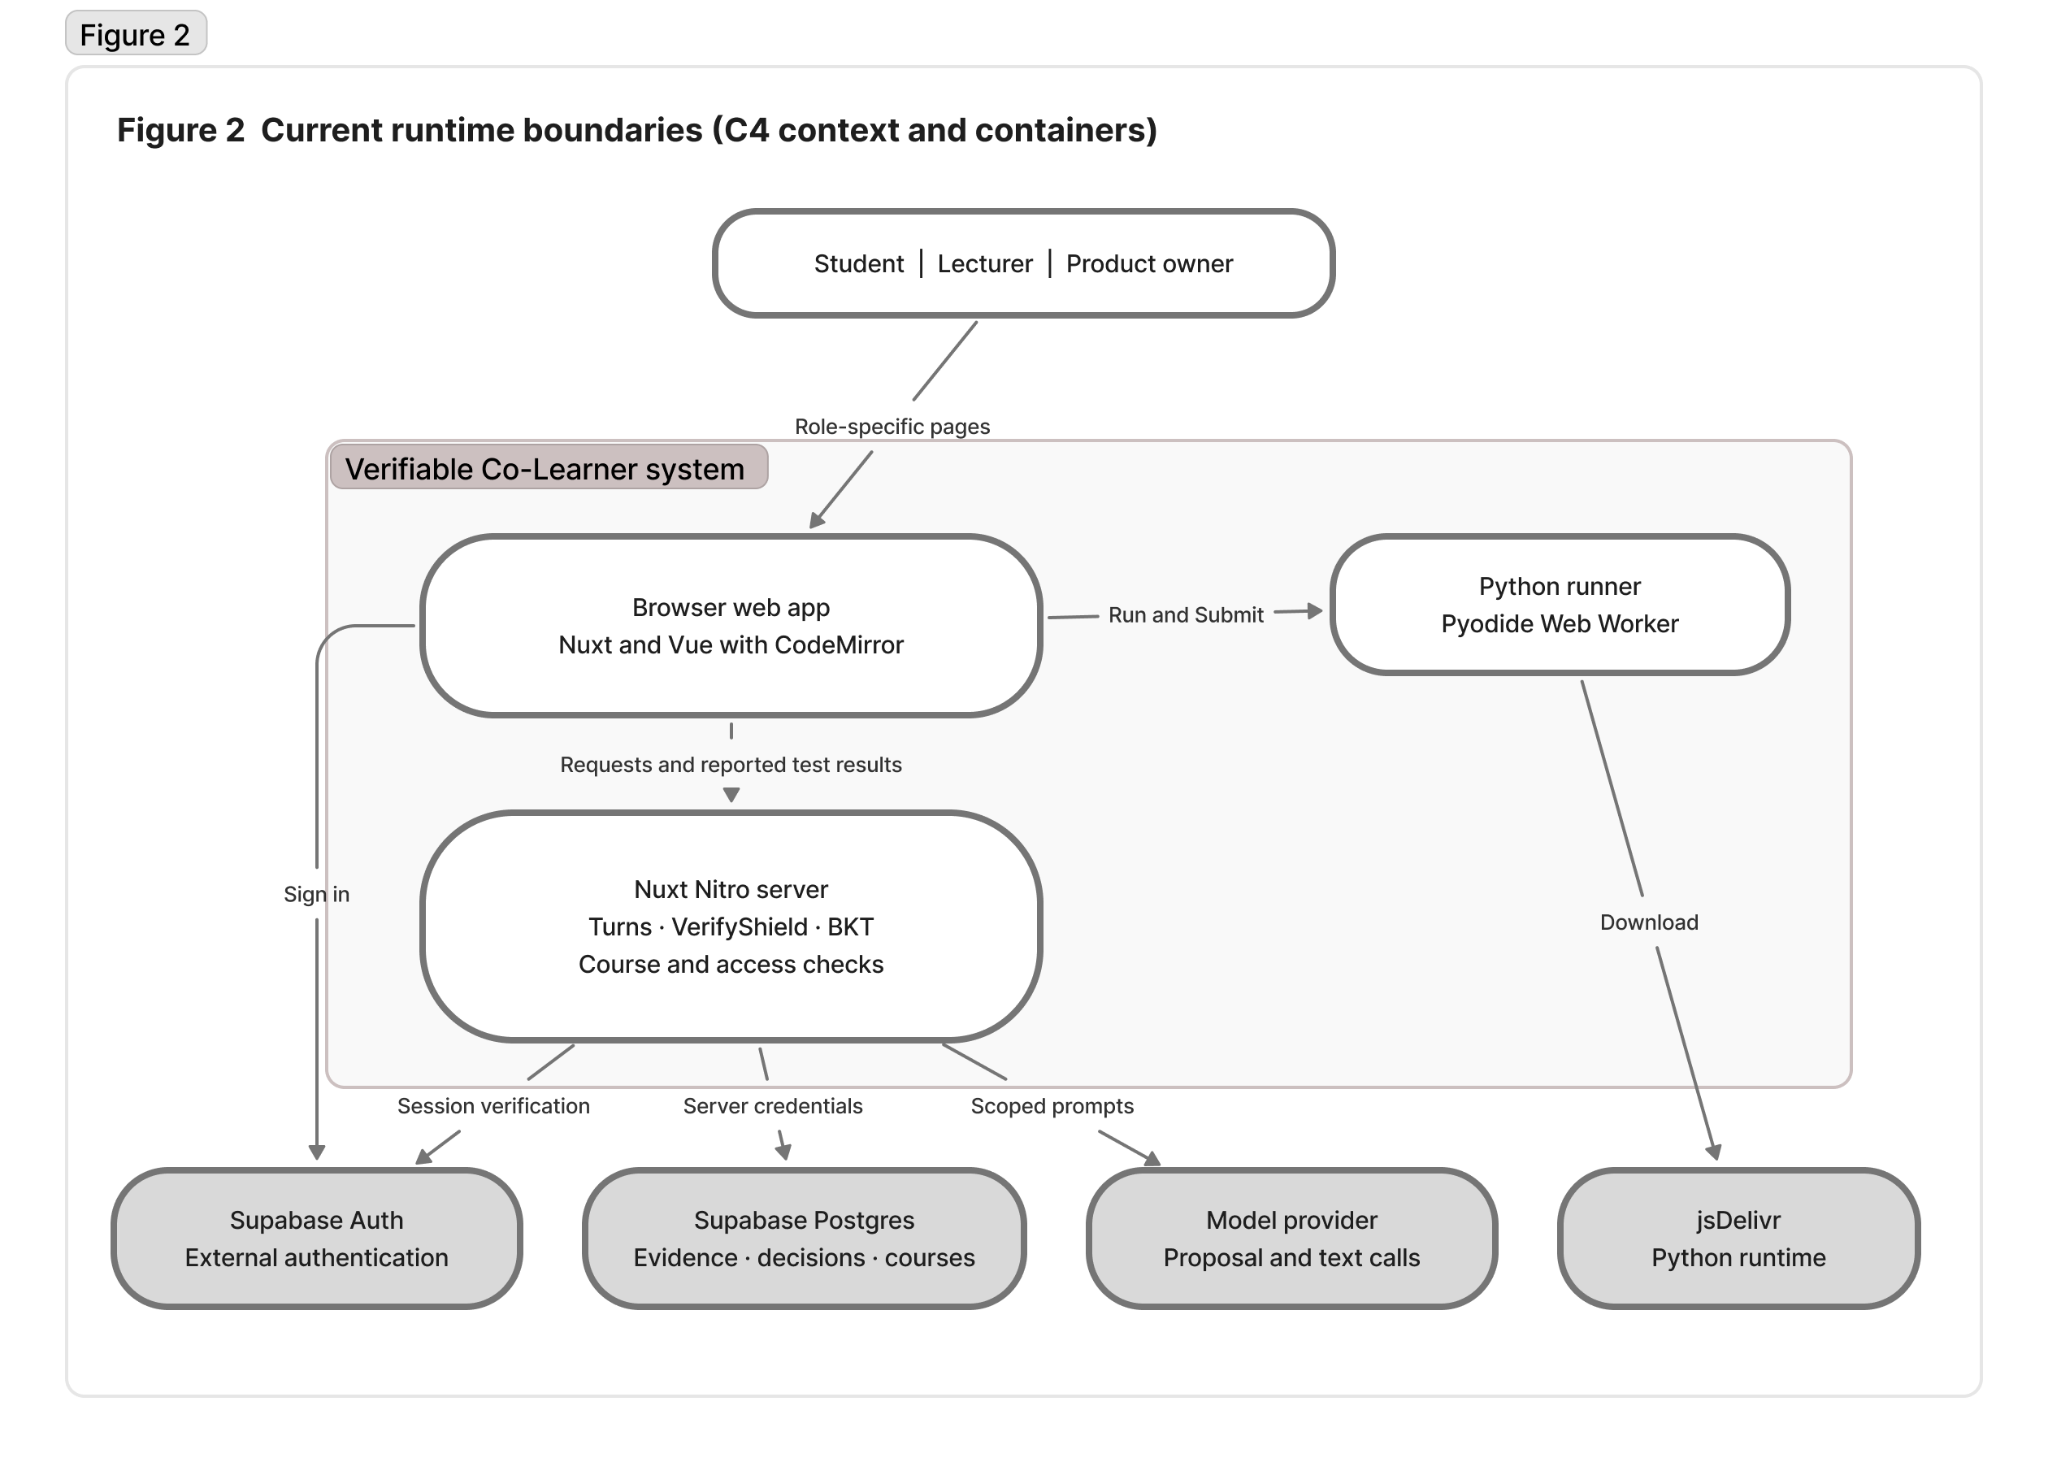
\includegraphics[width=0.90\linewidth]{figures/figure-1.png}
\caption{Sprint 1 runtime view, adapted from the repository's C4 Level 1 (system context) and Level 2 (container) diagrams.}
\end{figure}
\subsubsection{What the increment does}
In the web app container, the Study layout presents the roadmap, working area and conversation side by side, and the Roadmap layout arranges the same workspace on a draggable canvas. Drafts stay on the student's device, while resume points and one conversation per module persist through server storage. The Python runner container runs \textbf{Pyodide }in a Web Worker, so student code executes without blocking the interface.

On Submit, the browser sends the code and its test results to the turn and admin server. The server appends the test counts to the evidence ledger, updates the module's \textbf{Bayesian Knowledge Tracing (BKT)} estimate and records permanent unlocks. Quiz answers are marked on the server and also count toward mastery. A module is mastered when its estimate reaches the threshold and at least one of its exercises has passed.

\textbf{Supabase }provides authentication and the Postgres database, while the Nitro server owns data access, course interpretation, agent orchestration and the VerifyShield. Row-level security denies students direct access to the database, and the server reads and writes on their behalf with privileged credentials. \textbf{In Sprint 1 the application runs locally against the Supabase} and an external language model provider.

\subsection{Teamwork and delivery evidence}
{\footnotesize
\begin{longtable}{>{\raggedright\arraybackslash}p{\dimexpr 0.155\linewidth-2\tabcolsep\relax}>{\raggedright\arraybackslash}p{\dimexpr 0.214\linewidth-2\tabcolsep\relax}>{\raggedright\arraybackslash}p{\dimexpr 0.197\linewidth-2\tabcolsep\relax}>{\raggedright\arraybackslash}p{\dimexpr 0.166\linewidth-2\tabcolsep\relax}>{\raggedright\arraybackslash}p{\dimexpr 0.268\linewidth-2\tabcolsep\relax}}
\caption{Contribution by Jira responsibility and merged PR authorship, 26 October--15 November.}\\
\toprule
\textbf{Member } & \textbf{Role} & \textbf{Jira Done / assigned} & \textbf{Merged PRs in sprint} & \textbf{Evidence and interpretation} \\
\midrule
\endhead
Quoc Trung & Security Requirements & 7 / 7 & 2 & Security testing: prompt-injection probes and an LLM malware-injection breakdown in PR \#122 and PR \#123. This is substantive work despite the low PR count. \\
Duc Manh & Scrum and UX & 7 / 7 & 11 & Language-model switch (PR \#80) and the C4 documentation sync (PR \#157), alongside Scrum coordination. \\
Anh Tuan & Verification and quality & 7/ 7 & 36 & Workspace prototypes (PR \#31--32), the design pass (PR \#63--67 and PR \#69), the demo rehearsal (PR \#41) and model settings (PR \#107). Building most of the core reduces the independence of quality review. \\
Thuan Minh & Architecture & 7/ 7 & 8 & Agent navigation aligned with the glossary (PR \#142), the decision boundary check by turn ID (PR \#144), quiz mastery (PR \#150) and lecturer pages (PR \#166 and PR \#167). \\
Xuan Doanh & Ethics and board & 6 / 6 & 13 & Conversation and roadmap UI (PR \#113--121), the move and snapshot contracts (PR \#148) and prompt hardening (PR \#151, PR \#153, PR \#155). \\
\bottomrule
\end{longtable}}
\begin{figure}[H]
\centering
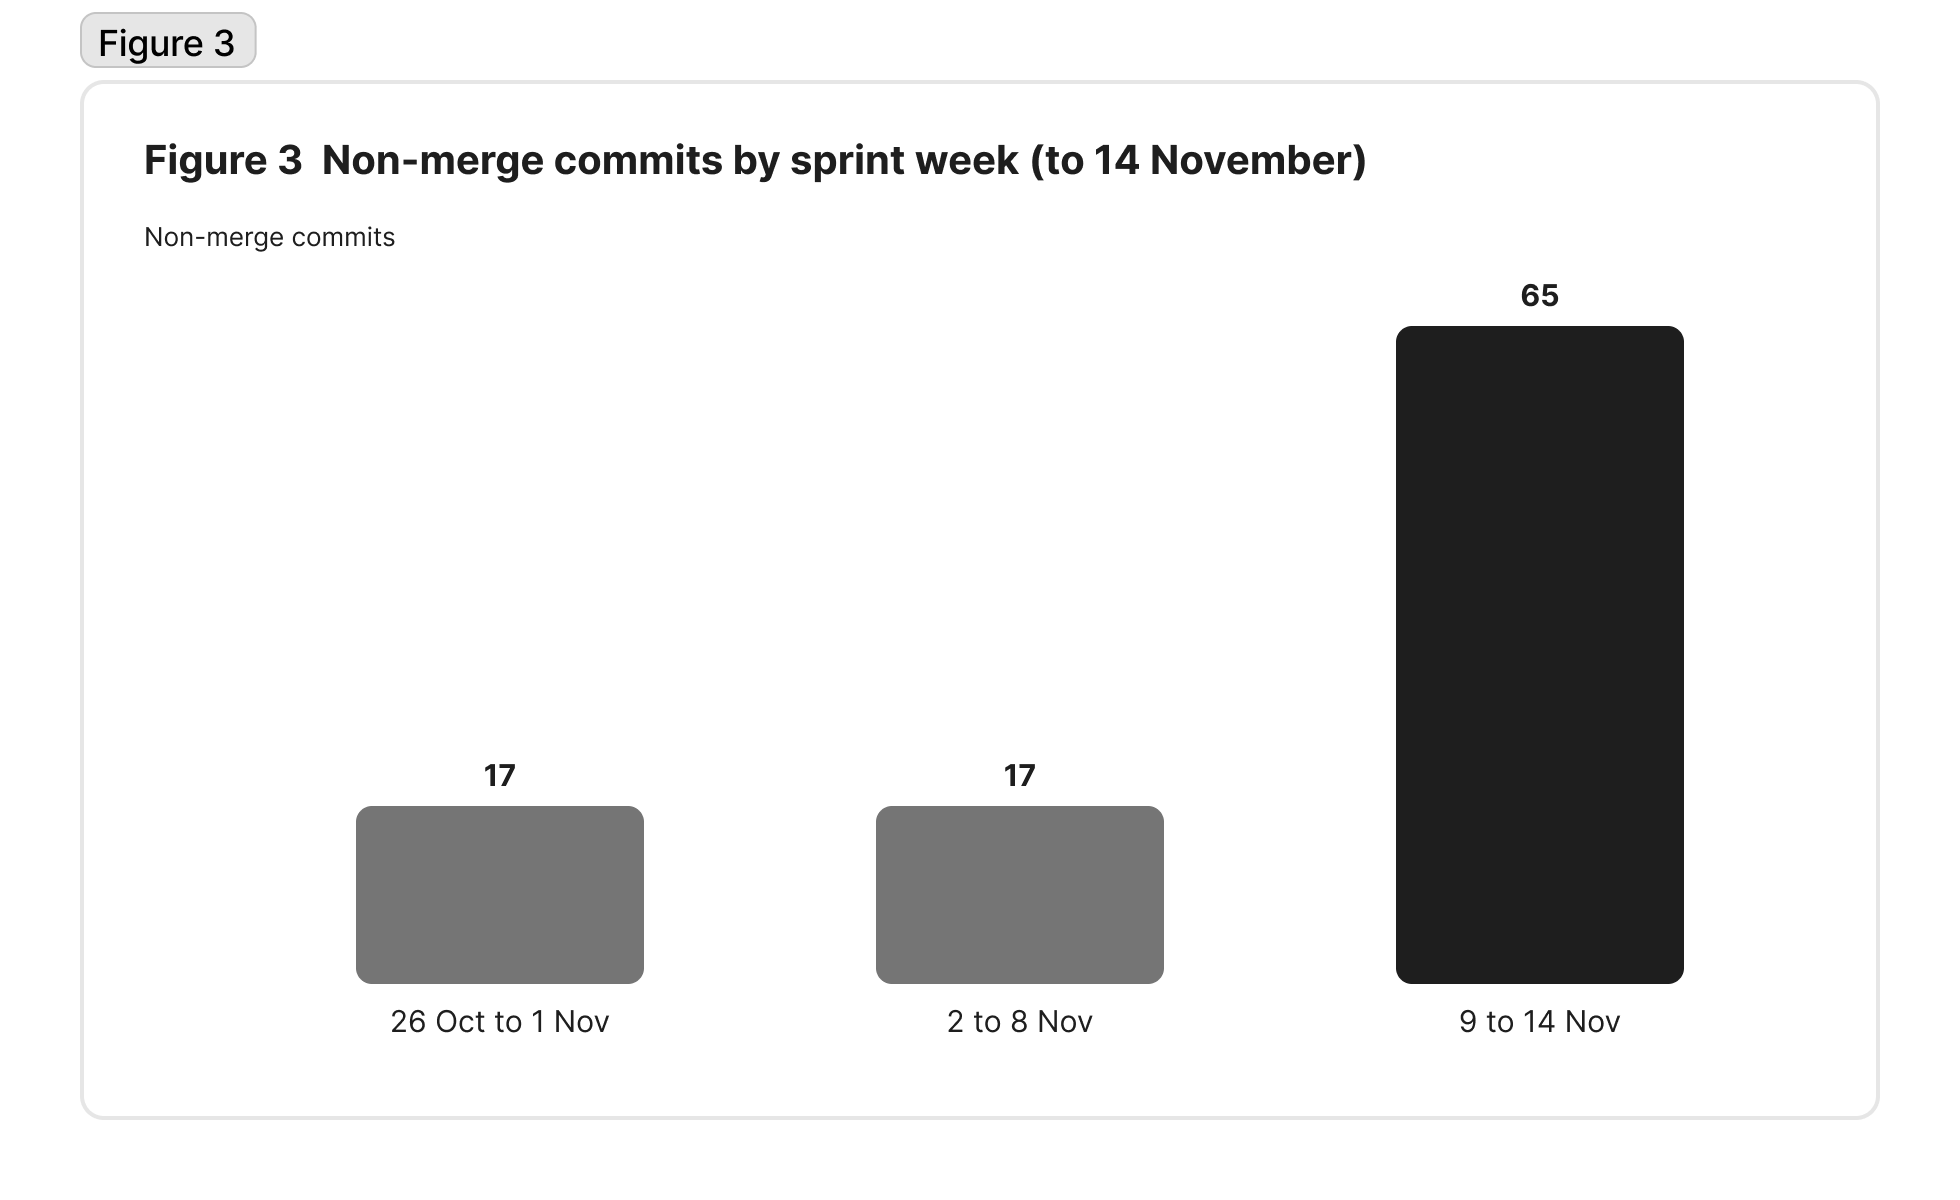
\includegraphics[width=0.84\linewidth]{figures/figure-2.png}
\caption{Non-merge commits by sprint week, counted by committer date. The final bar ends at the latest retrieved commit on 14 November.}
\end{figure}
The sprint contains 99 non-merge commits and 70 merged PRs. Repository-wide totals are 108 non-merge commits and 75 merged PRs; the earlier nine commits and five PRs are excluded from sprint totals. The last week contains 65 of 99 commits (65.7\%), which indicates concentrated integration and review pressure, not its cause.

\subsection{Testing results}
{\small
\begin{longtable}{>{\raggedright\arraybackslash}p{\dimexpr 0.250\linewidth-2\tabcolsep\relax}>{\raggedright\arraybackslash}p{\dimexpr 0.292\linewidth-2\tabcolsep\relax}>{\raggedright\arraybackslash}p{\dimexpr 0.458\linewidth-2\tabcolsep\relax}}
\caption{Test and security results on the main branch.}\\
\toprule
\textbf{Check} & \textbf{Result} & \textbf{What it shows} \\
\midrule
\endhead
Unit and integration tests & 303 passed, 11 failed & Ten failures are database tests that need a connection to the Supabase test project. The eleventh is a migration test that timed out and passes when run on its own. \\
End-to-end tests & 6 test files & Cover sign-in, the phone and tablet layouts, and a full rehearsal of the client demo. \\
Manual security testing & 89 attack prompts & No prompt made an agent write out the finished solution. Two issues were found: the Teacher could walk a student through the answer step by step, and test results sent from the browser could be faked. \\
Automated security checks & 7 of 7 live checks; 2 of 3 regression checks & The failed check is the answer-reveal issue found in manual testing, which was fixed afterwards. \\
\bottomrule
\end{longtable}}
The security testing changed the design. Once it showed that the Teacher could give away an answer, we removed the reveal-answer move, limited hints to three levels that must be used in order, and hardened the agents' prompts. Checking submitted test results on the server, so that they cannot be faked, is part of the Sprint 2 sandbox work.

\section{Sprint Review}
\subsection{Increment available for client review}
\textbf{The client live demonstration} took place on \textbf{12/Nov/2026} during the Project A lecturer time with the presence of \textbf{Dr. Le Minh Duc (project supervisor), Dr. Nguyen Manh Toan and other teams}. Therefore our sprint review will show the reviews we got from that demo and our own critical analysis.

\subsection{Demonstration session}
We \textbf{rehearsed }the demonstration with a \textbf{Playwright script} that signs in, opens the editor, runs and submits code, checks that both agents reply, and confirms that the student can resume where they left off. The script resets the demo accounts before each run, and a fake model is ready in case the live model provider or the network fails.

During the client demonstration, we followed the order in which a user meets the system. We signed in first as a student and then as the product owner (PO), showing that each role gets its own interface. As students, we wrote Python in the browser, ran it, submitted it and watched the \textbf{module's mastery rise} after a correct submission. We then asked the Teacher for help, including a prompt written to talk it into giving away the answer, to show how the \textbf{VerifyShield} handles that request. The PO then switched the \textbf{VerifyShield off} so the same question could be compared with and without it. Finally, the PO's dashboard showed each agent's decision in the decision log, with the proposal, the verdict and the reason.

\begin{figure}[H]
\centering
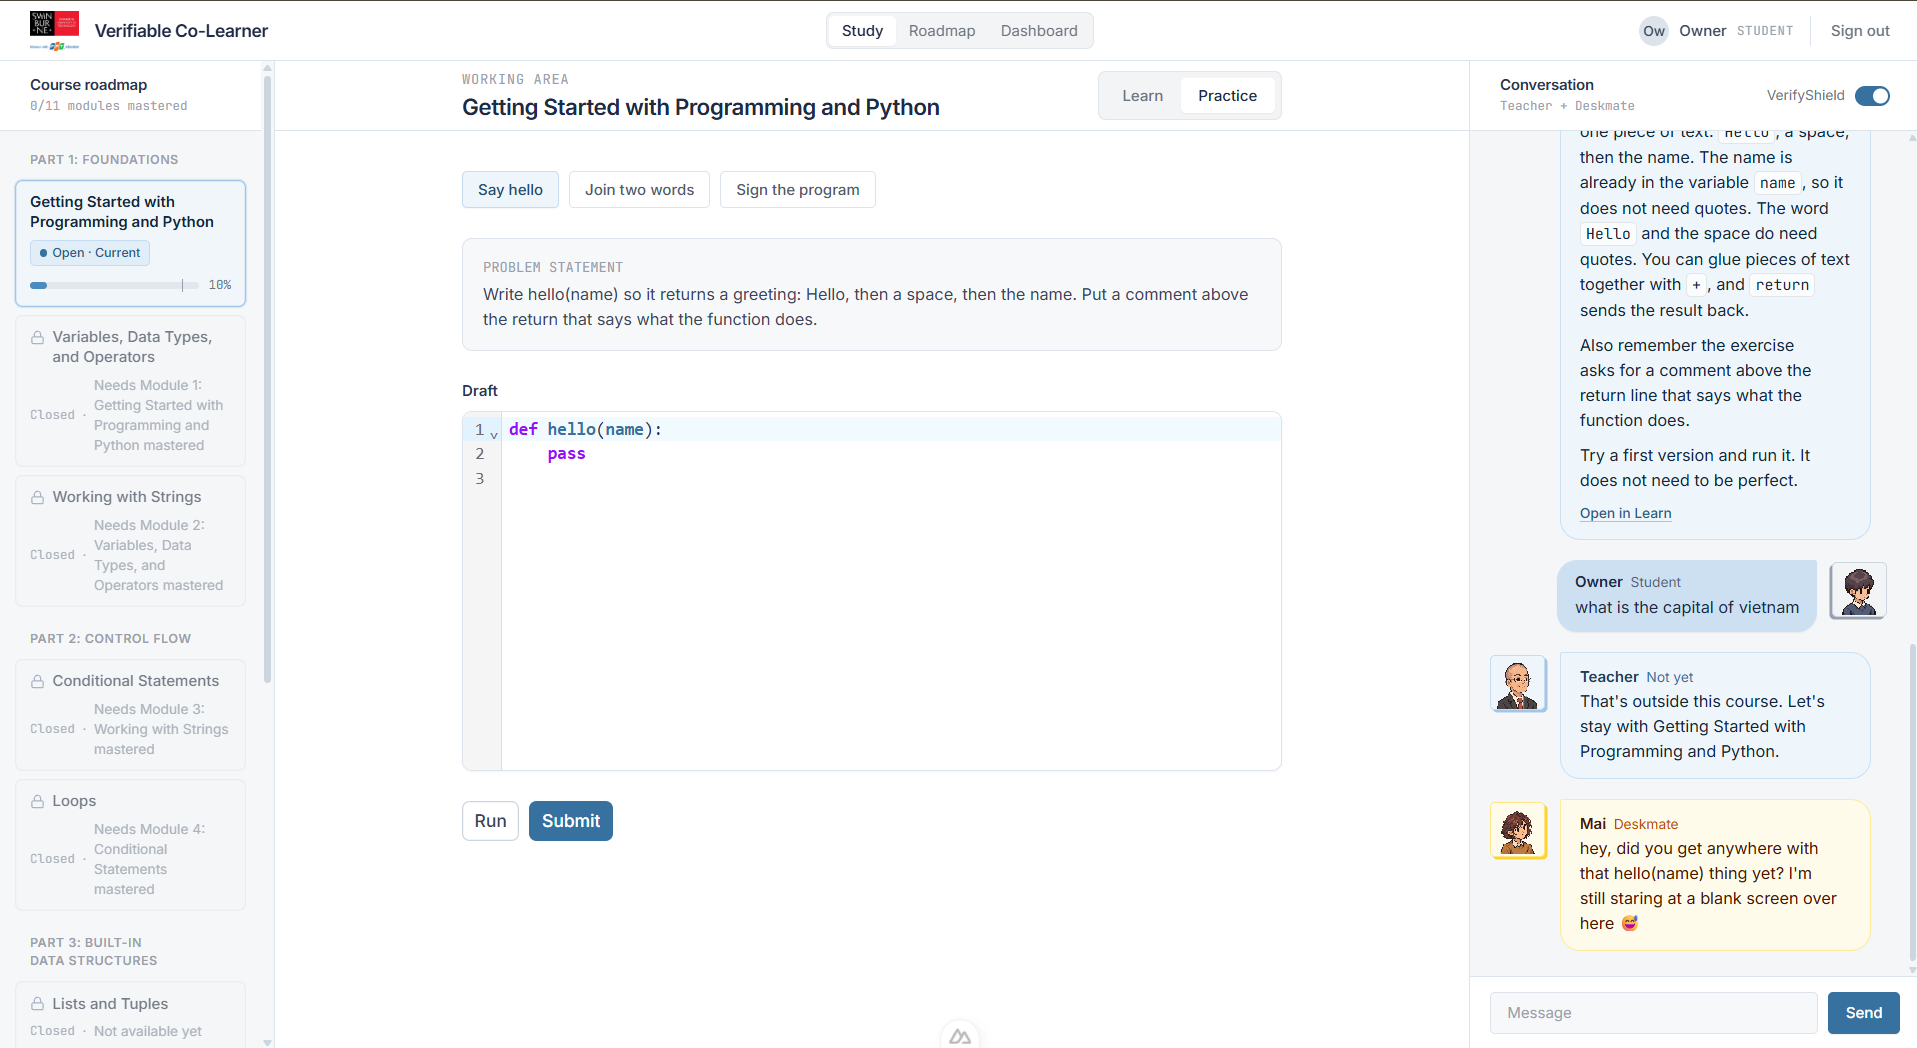
\includegraphics[width=0.95\linewidth]{figures/figure-3.png}
\caption{Practice workspace.}
\end{figure}
\begin{figure}[H]
\centering
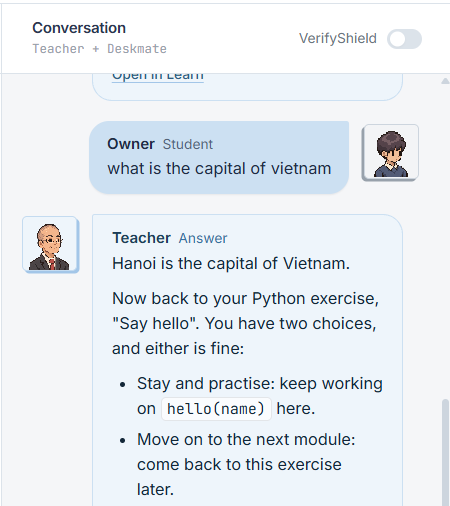
\includegraphics[width=0.56\linewidth]{figures/figure-4.png}
\caption{Agent replies with VerifyShield off.}
\end{figure}
\begin{figure}[H]
\centering
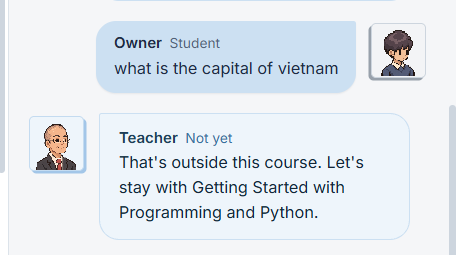
\includegraphics[width=0.76\linewidth]{figures/figure-5.png}
\caption{Agent reply with VerifyShield on.}
\end{figure}
\subsection{What VerifyShield proves}
\textbf{VerifyShield is what makes the system verifiable. Each agent first proposes a typed move, such as a hint at a given level or a redirect to another module, and deterministic rules rule on that move before any text is generated, so the same proposal and course state always produce the same verdict. Every ruling is written to the decision log with its rule and reason, and switching the shield off gives a baseline to compare against. In Sprint 1 the shield rules on the move, not on the wording the model writes for an approved move.}

\subsection{Critical analysis of our progress}
\subsubsection{The core goal is demonstrated by the implementation but not fully assured}
A1--A3 form a coherent end-to-end increment, supported by implementation, test source and merged changes. A4--A6 each deliver useful behaviour and all their Jira tasks are closed. The gaps below, also raised in Quoc Trung's Jira review on 14 November, are product-quality issues that Sprint 2 finishes.

{\small
\begin{longtable}{>{\raggedright\arraybackslash}p{\dimexpr 0.181\linewidth-2\tabcolsep\relax}>{\raggedright\arraybackslash}p{\dimexpr 0.140\linewidth-2\tabcolsep\relax}>{\raggedright\arraybackslash}p{\dimexpr 0.370\linewidth-2\tabcolsep\relax}>{\raggedright\arraybackslash}p{\dimexpr 0.309\linewidth-2\tabcolsep\relax}}
\caption{Gaps against the Sprint 1 goal.}\\
\toprule
\textbf{Gap and owner} & \textbf{Owner} & \textbf{Cause and practical effect} & \textbf{Resolution and acceptance evidence} \\
\midrule
\endhead
A4 Feedback & Quoc Trung & The panel prints Python error/stderr directly and still states that a submission is not recorded. The server now persists it, so the UI gives a misleading account of data use. & Translate common errors while preserving diagnostic detail; correct Run/Submit wording. Test a failing submission and inspect its persisted evidence. \\
A5 evidence trust & Quoc Trung with Anh Tuan research & ADR 0002 defers a second server run to avoid latency and parity costs. The API accepts browser-reported results, so a direct caller can manufacture mastery and permanent unlocks. & Choose authoritative verification with isolation and resource limits. A forged all-pass payload must not create a correct observation or unlock a module. \\
A6 audit integrity & Quoc Trung with Xuan Doanh research & The store exposes append and list, but the privileged database role can alter rows. The log lacks hashes and a complete versioned decision snapshot. & Add mutation controls and tamper detection; retain pinned decision inputs and versions. Verify modified-row detection and replay of allow, block and downgrade. \\
\bottomrule
\end{longtable}}
\subsubsection{Changes that improved the increment}
Course content moved into a validated database specification, lecturer settings became available, and quizzes added another evidence type. These reduce hard-coded course handling and make configuration visible. Their PRs show useful delivery, but no documented client change request proves why they displaced other work. Future additions should record both the value and the work deferred.

\subsubsection{Differences from the wider project plan}
The Week 6 plan called for post-render checking, trusted evidence producers, versioned replay and graph validation. Sprint 1 implements move checking, a linear course order, recorded unlocks and restricted log access. It does not yet deliver the full earlier verification architecture. Similarly, agents already react to module opening, submissions and wrong quiz answers; Sprint 2 is therefore an extension toward persistent plans and controlled initiative, not the first introduction of event-driven behaviour.

\subsection{Client review and acceptance record}
\subsubsection{Review session record}
{\small
\begin{longtable}{>{\raggedright\arraybackslash}p{\dimexpr 0.259\linewidth-2\tabcolsep\relax}>{\raggedright\arraybackslash}p{\dimexpr 0.741\linewidth-2\tabcolsep\relax}}
\caption{Review session record.}\\
\toprule
\textbf{Item} & \textbf{Detail} \\
\midrule
\endhead
Date and format & 12 November 2026, live demonstration during Project A lecture time \\
Reviewers & Dr. Le Minh Duc (supervisor), Dr. Nguyen Manh Toan and the other project teams \\
Demonstrated flows & All the flows in 3.2, in that order \\
Issue during the demo & Once, the Teacher answered a question about a locked module instead of redirecting the student \\
Acceptance & Accepted. Dr. Duc said the work was good and asked for more improvement in making the system a real AI agent \\
\bottomrule
\end{longtable}}
{\small
\begin{longtable}{>{\raggedright\arraybackslash}p{\dimexpr 0.333\linewidth-2\tabcolsep\relax}>{\raggedright\arraybackslash}p{\dimexpr 0.333\linewidth-2\tabcolsep\relax}>{\raggedright\arraybackslash}p{\dimexpr 0.333\linewidth-2\tabcolsep\relax}}
\caption{Feedback from the review and our response.}\\
\toprule
\textbf{Feedback} & \textbf{Our response} & \textbf{Sprint 2 item and owner} \\
\midrule
\endhead
Limit how much a student can chat (reviewers) & Each conversation already sends only the last 30 messages to the model, but there is no limit per student, which matters for cost and abuse on a public site. & A11: a per-student message limit before the test site goes live \\
Malware submitted through the chat or the practice workspace (reviewers) & Chat text is never executed, and practice code runs only in the student's browser today. Once the server runs submissions, harmful code must be contained. & A9: sandbox with no network or file access, plus harmful-code cases in the security tests \\
Security of the agents' access to the database (reviewers) & The agents have no direct database access: the server reads and writes for them, and row-level security blocks students. As the agents gain tools, each tool must be read-only and limited to the current student. & A7: least-privilege agent tools, with every tool call ruled on by VerifyShield \\
No detection of answers copied from outside (reviewers) & The system cannot yet tell when a student pastes a finished answer, so mastery could rise without real work. & A10: flag large pastes and sudden complete solutions, and have the Teacher ask the student to explain the code \\
Not yet a real agentic AI (Dr. Duc and reviewers) & We agree. The agents react to the student's actions but do not yet keep a plan or decide for themselves when to act. & A7: agents that observe, plan and act, with every action ruled on and logged \\
The Teacher answered a question about a locked module (observed during the demo) & The scope check relies on the model labelling the question correctly, and this phrasing got through. & A12: add the question to the benchmark as a regression case; A8 limits retrieved material to open modules \\
\bottomrule
\end{longtable}}
\section{Sprint Retrospect}
\subsection{Team and communication plans}
M1 and M2 record the two Sprint 1 team meetings: 3 November set scope, owners and dates; 10 November reviewed milestones, the shield edge case and security findings. Each lists attendance and the decisions behind the Jira cards

M1 Meeting minutes, Sprint 1 technical planning, 3 November 2026. Google Drive: https://bit.ly/3UA38br

M2 Meeting minutes, Sprint 1 progress review, 10 November 2026. Google Drive:

https://bit.ly/3WO9l42

{\small
\begin{longtable}{>{\raggedright\arraybackslash}p{\dimexpr 0.285\linewidth-2\tabcolsep\relax}>{\raggedright\arraybackslash}p{\dimexpr 0.338\linewidth-2\tabcolsep\relax}>{\raggedright\arraybackslash}p{\dimexpr 0.377\linewidth-2\tabcolsep\relax}}
\caption{Team and communication plans against what happened.}\\
\toprule
\textbf{Plan commitment} & \textbf{Observed outcome and analysis} & \textbf{Change for Sprint 2} \\
\midrule
\endhead
Shared ownership and two implementation tasks in progress per member & Anh Tuan wrote 36 of the 70 merged PRs, so the quality lead also built most of the core. The cause was sequencing: the turn flow and VerifyShield had to exist before anyone could build on them, and with no task breakdown until the final week, new work went to the member who already knew that code. & Duc Manh tracks weekly capacity. Thuan Minh and Xuan Doanh pair on core work, and another member reviews Anh Tuan's changes. \\
Friday Meet with written minutes; Messenger response within 24 hours & Meetings were held, but the minutes were not kept in one shared place. No member was named as note-keeper, so each organiser saved minutes in their own Drive. & Duc Manh keeps one meeting log with date, attendance, decisions and owners, linked from Jira. \\
Jira tasks with owner, due date and weekly status checks & The 34 sub-tasks were added near the end of the sprint without estimates or due dates, and the Jira sprint was never started. Planning happened in meetings and Messenger, and Jira was treated as a record to update afterwards rather than as the plan itself, so it never showed progress during the sprint. & Xuan Doanh starts Sprint 2 in Jira with estimates and links PRs to their cards. Duc Manh reviews status each week. \\
Warn of delay 24 hours ahead; use named backups & We did not log whether any delay was escalated or a backup stepped in. The plan named no place to record a warning or a hand-over, so any that happened stayed in Messenger. & Each carried-over task gets an agreed owner and reviewer at Sprint 2 planning. \\
\bottomrule
\end{longtable}}
\subsection{Quality plan and technical learning}
Small issue-linked pull requests, a shared glossary, five ADRs and a repeatable test setup kept the code easy to follow. The weak point was review: 64 of the 70 merged PRs were merged by their own author, with no recorded GitHub review. From Sprint 2, every PR needs approval from a member other than its author, with the test result and the Jira acceptance condition linked in the PR.

\subsection{Risk register revisited}
We reassessed the twelve risks from the Week 6 plan. Each score is likelihood $\times$ severity on a 1--5 scale, and 15 or above needs immediate action.

{\small
\begin{longtable}{>{\raggedright\arraybackslash}p{\dimexpr 0.230\linewidth-2\tabcolsep\relax}>{\raggedright\arraybackslash}p{\dimexpr 0.123\linewidth-2\tabcolsep\relax}>{\raggedright\arraybackslash}p{\dimexpr 0.227\linewidth-2\tabcolsep\relax}>{\raggedright\arraybackslash}p{\dimexpr 0.421\linewidth-2\tabcolsep\relax}}
\caption{Risk register after Sprint 1.}\\
\toprule
\textbf{Risk and } & \textbf{Owner} & \textbf{Old $\rightarrow$ proposed L$\times$S} & \textbf{Sprint evidence and next control} \\
\midrule
\endhead
R1 AWS access & Thuan Minh & 12 $\rightarrow$ 3$\times$4=12 & The demo runs on localhost, Supabase and DeepSeek. Sprint 2 deploys to a public test domain; AWS stays future work. \\
R2 Learner approval & Xuan Doanh & 12 $\rightarrow$ 3$\times$4=12 & Only demo accounts were used. Keep testing internal until the supervisor approves a study. \\
R3 Runner and result integrity & Thuan Minh & 15 $\rightarrow$ 4$\times$5=20 & Test results reported by the browser are trusted. In Sprint 2 a server-side sandbox re-runs every submission. \\
R4 Token cost & Thuan Minh & 12 $\rightarrow$ 3$\times$4=12 & The fake model, a 30-message cap and a single retry keep cost down. Add spend tracking and a hard limit. \\
R5 Provider privacy & Xuan Doanh & 15 $\rightarrow$ 3$\times$5=15 & Provider terms and data region still need review. Use synthetic input until that is done. \\
R6 Key person dependency & Duc Manh & 16 $\rightarrow$ 4$\times$5=20 & Core code depends heavily on Anh Tuan. Pair on the turn flow and VerifyShield so a second member can maintain them. \\
R7 Specification drift & Quoc Trung & 12 $\rightarrow$ 3$\times$4=12 & Course history and the stored threshold help. Next, store the course, rule and code versions with each decision. \\
R8 Member unavailable & Duc Manh & 9 $\rightarrow$ 3$\times$3=9 & No absences this sprint. Keep backups and handover notes. \\
R9 Delayed supervisor decision & Duc Manh & 9 $\rightarrow$ 3$\times$3=9 & No delay was traced to supervisor decisions. Keep logging open questions and the date a decision is needed. \\
R10 Evidence loss or document conflict & Xuan Doanh & 9 $\rightarrow$ 3$\times$3=9 & Code is safe in Git, but meeting and acceptance records are scattered. Keep one evidence index. \\
R11 Competing assignments & Duc Manh & 12 $\rightarrow$ 4$\times$3=12 & 65.7\% of commits landed in the final week. Add a mid-sprint integration checkpoint. \\
R12 Story coverage & Quoc Trung & 12 $\rightarrow$ 3$\times$4=12 & Requirement-to-task links held. The exercise-authoring form (CH9VSA-93) remains a separate story. \\
\bottomrule
\end{longtable}}
\subsection{Ethics, privacy and new risks}
{\small
\begin{longtable}{>{\raggedright\arraybackslash}p{\dimexpr 0.450\linewidth-2\tabcolsep\relax}>{\raggedright\arraybackslash}p{\dimexpr 0.550\linewidth-2\tabcolsep\relax}}
\caption{New risks from this sprint.}\\
\toprule
\textbf{Risk and score} & \textbf{Control and accountable owner} \\
\midrule
\endhead
R13 Tracker drift \newline 4$\times$3 = 12 & Xuan Doanh links Jira acceptance to PR evidence and captures a sprint baseline on 16 Nov. \\
R14 Unrecorded independent review \newline 4$\times$4 = 16 & Duc Manh assigns a non-author reviewer and verifies approval before merging from 16 Nov. \\
R15 Additional scope displaces Must work \newline 3$\times$4 = 12 & Quoc Trung records the value, cost and displaced item before adding work; client/supervisor scope decisions go into minutes. \\
\bottomrule
\end{longtable}}
\subsubsection{Ethical protocol review}
Sprint 1 used only seeded demo accounts and internal security tests, with no real students. The plan's limits still apply: no monitoring of exams, webcams, keystrokes or unrelated learning systems. The table below checks the plan's privacy commitments against the Australian Privacy Principles (APPs).

{\small
\begin{longtable}{>{\raggedright\arraybackslash}p{\dimexpr 0.273\linewidth-2\tabcolsep\relax}>{\raggedright\arraybackslash}p{\dimexpr 0.364\linewidth-2\tabcolsep\relax}>{\raggedright\arraybackslash}p{\dimexpr 0.364\linewidth-2\tabcolsep\relax}}
\caption{Privacy commitments against the Australian Privacy Principles.}\\
\toprule
\textbf{Protocol commitment} & \textbf{Current implementation and gap} & \textbf{Required follow-up} \\
\midrule
\endhead
Transparent collection \newline APP 1 and APP 5 themes & No privacy notice at first login yet. & Xuan Doanh drafts the notice before any pilot. \\
Minimum necessary data \newline APP 3 and APP 4 themes & Prompts leave out email and name, but code and chat text can still identify a student. & Xuan Doanh and Thuan Minh review what is sent to the model and test for identifiers. \\
Overseas processing \newline APP 8 theme & Supabase and the model provider are external services, and their data regions are not yet recorded. & Xuan Doanh records the provider, region and handling rules. Use synthetic input until then. \\
Security and retention \newline APP 11 theme & Row-level security limits what students can access. The 30-day and 12-month retention limits are still to be built. & Thuan Minh and Xuan Doanh add retention and deletion jobs. \\
Learner agency and contestability & Hints are graduated and mastery is not a grade. There is no appeal process or accessibility audit yet. & Duc Manh and Anh Tuan test keyboard use and set up a human review process before a pilot. \\
\bottomrule
\end{longtable}}
\section{Reflection and Sprint 2 Priorities}
The review confirmed that \textbf{the core idea works}. Dr. Duc accepted the increment, and the reviewers saw each agent move ruled on by \textbf{VerifyShield }before the student saw it. Their questions also showed that we had looked at verification too narrowly. We had focused on what the agents say, while the reviewers asked about everything around it: how much a student can send, what happens to harmful code, what the agents can reach in the database, and whether a pasted answer should count as learning. The locked-module question the Teacher answered during the demo made the same point from inside the system: a rule we had not tested against that phrasing let the reply through.

The clearest message was that the system still behaves like a chatbot. In Sprint 1 the agents mostly respond to the student; they do not keep a plan or decide for themselves when to step in. Sprint 2 therefore puts the agentic work first and pairs it with the safeguards the reviewers asked for, so new capability and new protection arrive together. Two process lessons carry over as well (4.1 and 4.2): the Jira sprint must be set up before work starts, and every change needs a reviewer other than its author.

\textbf{Lessons learned from Sprint 1, each with the action we are taking:}

\begin{enumerate}
\item Plan in Jira before building. The 34 sub-tasks were entered after the work, so progress could not be tracked mid-sprint. Xuan Doanh starts Sprint 2 in Jira on 16 November with every item estimated (Table 14).
\item Every change needs a second reviewer. 64 of the 70 merged PRs were merged by their own author. From 16 November each PR needs a non-author approval, and Duc Manh checks this weekly.
\item Integrate in the middle of the sprint, not at the end. 65.7\% of commits landed in the final week. On 26 November the demo rehearsal must pass on the main branch.
\item Test the shield against real student phrasing. The locked-module answer got through because the rule had only been tested on our own wording. The demo question and a 25-prompt benchmark (A12) are in place before A7 changes agent behaviour.
\item Never trust results computed in the browser. Security testing showed that submitted test results could be forged. The A9 sandbox comes first, and mastery updates only from server-verified results.
\item Share the core so no member is a bottleneck. Thuan Minh and Xuan Doanh pair with Anh Tuan on the turn flow and VerifyShield, and core PRs are reviewed by someone other than their author.
\end{enumerate}
\subsection{Sprint 2 backlog plan}
{\footnotesize
\begin{longtable}{>{\raggedright\arraybackslash}p{\dimexpr 0.179\linewidth-2\tabcolsep\relax}>{\raggedright\arraybackslash}p{\dimexpr 0.144\linewidth-2\tabcolsep\relax}>{\raggedright\arraybackslash}p{\dimexpr 0.144\linewidth-2\tabcolsep\relax}>{\raggedright\arraybackslash}p{\dimexpr 0.280\linewidth-2\tabcolsep\relax}>{\raggedright\arraybackslash}p{\dimexpr 0.252\linewidth-2\tabcolsep\relax}}
\caption{Sprint 2 backlog.}\\
\toprule
\textbf{Item} & \textbf{Owner} & \textbf{Estimate and target} & \textbf{What it delivers} & \textbf{Done when} \\
\midrule
\endhead
A7 Agentic AI system & Xuan Doanh, paired with Anh Tuan & 8 pts; by 4 Dec & Agents act on what they observe (a failed submission, a wrong quiz answer, a stalled student), keep an agreed plan across turns, and use read-only tools limited to the current student. & An agent acts without a student message, follows the agreed plan across reloads, and each action has a verdict in the decision log. \\
A8 RAG on coursework & Quoc Trung & 8 pts; by 2 Dec & Teacher and Mai replies draw on the lesson text, examples and exercises of the student's open modules. & Replies use the current module's material and never a closed module's. \\
A9 Sandboxed Python practice & Anh Tuan & 8 pts; by 25 Nov & The server re-runs each submission in a sandbox with time and memory limits and no network or file access, and explains errors in plain language. & Forged browser results are rejected and student code cannot reach the network or file system. \\
A10 Misconception recognition & Duc Manh & 5 pts; by 4 Dec & Each module lists its common mistakes; the agents detect and answer that exact mistake, and large pastes are flagged for the Teacher to question. & Each of Modules 1--5 has at least one mistake detected and answered specifically. \\
A11 Public test deployment & Duc Manh & 5 pts; by 2 Dec & The app runs on a public test domain with HTTPS, working sign-in and a per-student message limit, without AWS. & Testers sign in on the public URL and the demo rehearsal passes there. \\
A12 Evaluation and tamper-evident log & Thuan Minh & 8 pts; benchmark by 22 Nov, all by 6 Dec & A shield-on/off benchmark of 25 prompts that includes the locked-module question from the demo, a decision log that shows any edit, and a full test suite that runs in CI. & The benchmark runs with one command, an edited log row is detected, and no tests fail. \\
\bottomrule
\end{longtable}}
\clearpage
\phantomsection\addcontentsline{toc}{section}{References}
\begin{thebibliography}{9}
\bibitem{c4model} S. Brown, ``The C4 model for visualising software architecture.'' c4model.com. Accessed: Nov. 15, 2026. [Online]. Available: \url{https://c4model.com/}
\bibitem{repo} Group HN9, ``COS40005\_HN9\_Verifiable\_Co-Learner\_Agent,'' GitHub repository. Accessed: Nov. 15, 2026. [Online]. Available: \url{https://github.com/Bill2926/COS40005_HN9_Verifiable_Co-Learner_Agent}
\end{thebibliography}
\appendix
\section{Jira Task Traceability}
All 34 Sprint 1 sub-tasks with their Jira owner, status (D = Done) and the pull requests or files that implement them.

\subsection{Web app and editor}
{\small
\begin{longtable}{>{\raggedright\arraybackslash}p{\dimexpr 0.480\linewidth-2\tabcolsep\relax}>{\raggedright\arraybackslash}p{\dimexpr 0.080\linewidth-2\tabcolsep\relax}>{\raggedright\arraybackslash}p{\dimexpr 0.040\linewidth-2\tabcolsep\relax}>{\raggedright\arraybackslash}p{\dimexpr 0.400\linewidth-2\tabcolsep\relax}}
\toprule
\textbf{Jira sub-task} & \textbf{Owner} & \textbf{State} & \textbf{Evidence or remaining acceptance gap} \\
\midrule
\endhead
CH9VSA-111 \newline A1.1 CodeMirror editor with Run and Submit & Quoc Trung & D & PR \#33; PythonEditor.vue \\
CH9VSA-112 \newline A1.2 Pyodide browser runner in a Web Worker & Xuan Doanh & D & PR \#33; browser-runner.ts \\
CH9VSA-113 \newline A1.3 Responsive IDE and Roadmap canvas layouts & Duc Manh & D & PR \#91; PR \#93; PR \#96 \\
CH9VSA-133 \newline R1 Research Pyodide worker runtime and CodeMirror 6 editor & Duc Manh & D & Related code: editor and Python worker \\
CH9VSA-139 \newline R7 Research practice runner test semantics, shared namespace, and failure messages & Xuan Doanh & D & Related code: pyodide-session.mjs and runner tests \\
\bottomrule
\end{longtable}}
\subsection{Sign-in and saved progress}
{\small
\begin{longtable}{>{\raggedright\arraybackslash}p{\dimexpr 0.496\linewidth-2\tabcolsep\relax}>{\raggedright\arraybackslash}p{\dimexpr 0.083\linewidth-2\tabcolsep\relax}>{\raggedright\arraybackslash}p{\dimexpr 0.041\linewidth-2\tabcolsep\relax}>{\raggedright\arraybackslash}p{\dimexpr 0.380\linewidth-2\tabcolsep\relax}}
\toprule
\textbf{Jira sub-task} & \textbf{Owner} & \textbf{State} & \textbf{Evidence or remaining acceptance gap} \\
\midrule
\endhead
CH9VSA-114 \newline A2.1 Supabase sign-in and signed-in middleware & Thuan Minh & D & PR \#34; signed-in.ts \\
CH9VSA-115 \newline A2.2 Resume point and one conversation per module & Duc Manh & D & PR \#36; conversation-store.ts \\
CH9VSA-118 \newline A2.3 Drafts in localStorage and layout per device & Duc Manh & D & drafts/store.ts; workspace-layout.ts \\
CH9VSA-134 \newline R2 Research Supabase SSR auth, RLS-scoped reads, and resume persistence & Duc Manh & D & Related code: auth and conversation stores \\
CH9VSA-140 \newline R8 Research authorisation boundaries and RLS across student, lecturer and admin routes & Thuan Minh & D & Related code: access routes and boundary tests \\
\bottomrule
\end{longtable}}
\subsection{Teacher and deskmate chat}
{\small
\begin{longtable}{>{\raggedright\arraybackslash}p{\dimexpr 0.500\linewidth-2\tabcolsep\relax}>{\raggedright\arraybackslash}p{\dimexpr 0.067\linewidth-2\tabcolsep\relax}>{\raggedright\arraybackslash}p{\dimexpr 0.042\linewidth-2\tabcolsep\relax}>{\raggedright\arraybackslash}p{\dimexpr 0.392\linewidth-2\tabcolsep\relax}}
\toprule
\textbf{Jira sub-task} & \textbf{Owner} & \textbf{State} & \textbf{Evidence or remaining acceptance gap} \\
\midrule
\endhead
CH9VSA-116 \newline A3.1 Both agents propose in the same turn & Anh Tuan & D & PR \#38; PR \#116; handle-turn.ts \\
CH9VSA-117 \newline A3.2 Role table enforces the teacher/deskmate split & Anh Tuan & D & PR \#37; role-table.ts; decide.ts \\
CH9VSA-119 \newline A3.3 Conversation panel renders approved moves & Anh Tuan & D & PR \#68; ConversationPanel.vue \\
CH9VSA-135 \newline R3 Research typed agent moves and prompt-injection hardening for two-agent turns & Anh Tuan & D & PR \#146; PR \#153; prompts.ts \\
CH9VSA-141 \newline R9 Research language-model provider integration, structured output fallback and prompt budget & Duc Manh & D & Related code: provider adapter and prompt tests \\
\bottomrule
\end{longtable}}
\subsection{Practice with tests and plain-language errors}
{\small
\begin{longtable}{>{\raggedright\arraybackslash}p{\dimexpr 0.444\linewidth-2\tabcolsep\relax}>{\raggedright\arraybackslash}p{\dimexpr 0.074\linewidth-2\tabcolsep\relax}>{\raggedright\arraybackslash}p{\dimexpr 0.037\linewidth-2\tabcolsep\relax}>{\raggedright\arraybackslash}p{\dimexpr 0.444\linewidth-2\tabcolsep\relax}}
\toprule
\textbf{Jira sub-task} & \textbf{Owner} & \textbf{State} & \textbf{Evidence or remaining acceptance gap} \\
\midrule
\endhead
CH9VSA-120 \newline A4.1 45 checks across 5 modules x 3 exercises x 3 tests & Anh Tuan & D & PR \#111; course/modules; PracticePanel.vue \\
CH9VSA-121 \newline A4.2 Persist every submission as evidence & Anh Tuan & D & PR \#112; handle-turn.ts; evidence store \\
CH9VSA-122 \newline A4.3 Replace raw Python errors with plain-language messages & Quoc Trung & D & Done in Jira; full plain-language translation completes in Sprint 2 (A9) \\
CH9VSA-123 \newline A4.4 Fix the stale not-recorded-as-evidence copy & Quoc Trung & D & Done in Jira; the wording fix ships with Sprint 2 (A9) \\
CH9VSA-136 \newline R4 Research BKT mastery update, evidence ledger, and plain-language error taxonomy & Xuan Doanh & D & Related code: estimate.ts and evidence ledger \\
CH9VSA-142 \newline R10 Research browser and server Python parity for evidence verification & Anh Tuan & D & Findings recorded in ADR 0002; server re-run scheduled as A9 \\
\bottomrule
\end{longtable}}
\subsection{Shield core: hints, no early answers, topics open on mastery}
{\small
\begin{longtable}{>{\raggedright\arraybackslash}p{\dimexpr 0.444\linewidth-2\tabcolsep\relax}>{\raggedright\arraybackslash}p{\dimexpr 0.074\linewidth-2\tabcolsep\relax}>{\raggedright\arraybackslash}p{\dimexpr 0.037\linewidth-2\tabcolsep\relax}>{\raggedright\arraybackslash}p{\dimexpr 0.444\linewidth-2\tabcolsep\relax}}
\toprule
\textbf{Jira sub-task} & \textbf{Owner} & \textbf{State} & \textbf{Evidence or remaining acceptance gap} \\
\midrule
\endhead
CH9VSA-124 \newline A5.1 Scope gating, redirects, keyword backstop, fail-closed & Thuan Minh & D & PR \#108; PR \#109; PR \#156 \\
CH9VSA-125 \newline A5.2 BKT mastery and permanent module unlocking & Thuan Minh & D & PR \#112; PR \#143; PR \#167 \\
CH9VSA-126 \newline A5.3 Add an attempt or evidence gate for reveal\_answer & Thuan Minh & D & PR \#146; reveal\_answer removed from schema \\
CH9VSA-127 \newline A5.4 Cap hint\_level\_N and tie hints to attempts & Thuan Minh & D & PR \#152; hint history gate, not attempts \\
CH9VSA-128 \newline A5.5 Decide and schedule server-side verification of reported results & Quoc Trung & D & Decision recorded in ADR 0002; the server sandbox is planned for Sprint 2 \\
CH9VSA-137 \newline R5 Research adversarial prompt testing of the VerifyShield and rule coverage & Quoc Trung & D & Security report in PR \#122--123 \\
CH9VSA-143 \newline R11 Research hint ladder, misconception and keyword rule coverage on real phrasing & Thuan Minh & D & Related code: decide.test.ts; real-phrasing cases continue in A12 \\
\bottomrule
\end{longtable}}
\subsection{Course spec and decision log}
{\small
\begin{longtable}{>{\raggedright\arraybackslash}p{\dimexpr 0.444\linewidth-2\tabcolsep\relax}>{\raggedright\arraybackslash}p{\dimexpr 0.074\linewidth-2\tabcolsep\relax}>{\raggedright\arraybackslash}p{\dimexpr 0.037\linewidth-2\tabcolsep\relax}>{\raggedright\arraybackslash}p{\dimexpr 0.444\linewidth-2\tabcolsep\relax}}
\toprule
\textbf{Jira sub-task} & \textbf{Owner} & \textbf{State} & \textbf{Evidence or remaining acceptance gap} \\
\midrule
\endhead
CH9VSA-129 \newline A6.1 Decision log fields and admin filters & Xuan Doanh & D & PR \#109; decision-log.ts; admin.vue \\
CH9VSA-130 \newline A6.2 RLS and append-only store enforcement & Xuan Doanh & D & Decision migration; server append/list API \\
CH9VSA-131 \newline A6.3 Add a hash chain or DB-level append-only guard & Quoc Trung & D & Done in Jira; the hash chain is built in Sprint 2 (A12) \\
CH9VSA-132 \newline A6.4 Add runtime validation or one validated course spec & Duc Manh & D & PR \#164; PR \#168; parse-course-spec.ts \\
CH9VSA-138 \newline R6 Research course graph traversal, spec validation, and tamper-evident log design & Quoc Trung & D & Course and log design recorded in the ADRs \\
CH9VSA-144 \newline R12 Research decision-log replay determinism and tamper evidence & Xuan Doanh & D & Related code: decision-log store; replay and tamper evidence built in A12 \\
\bottomrule
\end{longtable}}
\section{AI Usage Disclosure}
The unit outline asks every team to declare how AI was used. The table below lists the AI used inside the product and the AI tools the team used during Sprint 1.

{\small
\begin{longtable}{>{\raggedright\arraybackslash}p{\dimexpr 0.333\linewidth-2\tabcolsep\relax}>{\raggedright\arraybackslash}p{\dimexpr 0.333\linewidth-2\tabcolsep\relax}>{\raggedright\arraybackslash}p{\dimexpr 0.333\linewidth-2\tabcolsep\relax}}
\toprule
\textbf{AI tool} & \textbf{What it was used for} & \textbf{How the team checked it} \\
\midrule
\endhead
Product language model (DeepSeek by default; a fake model for demos) & Writes the Teacher and Mai replies inside the app & VerifyShield rules on every proposed move and records it in the decision log \\
AI coding assistants (Claude Code, OpenAI Codex) & Drafting code, tests and documentation during development & The member who opened each pull request reviewed and integrated the output \\
AI chat assistants (Claude, ChatGPT) & Checking Jira and GitHub figures and drafting and restructuring sections of this report & The team checked every figure against Jira and GitHub and edited the wording \\
\bottomrule
\end{longtable}}
\end{document}
